
\documentclass[a4paper,12pt]{report}
\usepackage{xcolor}
\usepackage[unicode]{hyperref}
\hypersetup{colorlinks=true, urlcolor=green, linkcolor=black, unicode=true}
\usepackage[utf8]{vietnam}
\usepackage{latexsym, amsfonts, amssymb, amsmath}
\usepackage[margin=2.2cm]{geometry}
\usepackage{fancybox}
\usepackage{minted}
\usepackage{frame}
\usepackage{graphicx}
\begin{document}
	\thispagestyle{empty}
	\thisfancypage{
		\setlength{\fboxsep}{0pt}
		\fbox}{} 
	\begin{center}
		\begin{large}
			\textcolor[rgb]{1.00,0.00,0.00}{TRƯỜNG ĐẠI HỌC BÁCH KHOA HÀ NỘI}
		\end{large} \\
		\begin{large}
			\textcolor[rgb]{1.00,0.00,0.00}{VIỆN CÔNG NGHỆ THÔNG TIN VÀ TRUYỀN THÔNG}
		\end{large} \\
	
		\textbf{--------------------  *  ---------------------}\\[2cm]
	
		
\includegraphics[width=3cm, height=4.2cm]{logo}\\[1cm]
		{\fontsize{32pt}{1}\selectfont BÀI TẬP MÔN HỌC}\\
		{\fontsize{20pt}{1}\selectfont TOÁN RỜI RẠC}\\[2cm]
	\end{center}
	
	\hspace{5cm}  Đề tài 10 : Đường đi ngắn nhất trên đồ thị
	\begin{flushright}
		\parbox[t]{8cm}{
		\textbf{Nguyễn Duy Thành-}CNTT1 20102737\\
                \textbf{Vũ Văn Hiệp-}CNTT2 20101545}\\[12pt]
		%\textbf{Bạch Văn Hải-}CNTT1 20101464}\\[12pt]
	\end{flushright}
	
	\hspace{5cm} Giáo viên\hspace{24pt} :
	\begin{flushright} \textbf{\parbox[t]{8cm}{    
		\textcolor[rgb]{0.00,0.00,1.00}{Huỳnh Thanh Bình}
		}}
	\end{flushright}
	\vspace{2cm}
	\begin{center}
		{\fontsize{16pt}{1}\selectfont HÀ NỘI}\\
		{\fontsize{16pt}{1}\today}
	\end{center}
	
	\newpage

	\tableofcontents
	\newpage
\chapter*{Lời nói đầu}



		Trong lý thuyết đồ thị, bài toán tìm đường đi ngắn nhất giữa hai đỉnh của một đồ thị liên thông là một trong những bài toán có ứng dụng thực tế to lớn nhất. Từ bài toán này, người ta đã phát triển thành nhiều bài toán khác như: Bài toán chọn hành trình tiết kiệm nhất về thời gian, chi phí hay khoảng cách trên một mạng lưới giao thông; Bài toán lập lịch thi công các công đoạn của một công trình lớn, Bài toán lực chọn con đường truyền tin với chi phí thấp nhất trong mạng lưới thông tin, Bài toán tìm lời dịch tốt nhất cho một câu nói \ldots Đến nay, chúng ta đã có rất nhiều thuật toán để giải Bài toán tìm đường đi ngắn nhất với khả năng áp dụng và độ phức tạp khác nhau. Trong bài báo cáo này, chúng em xin trình bày về 6 phương pháp giải quyết bài toán này kèm theo project minh họa việc giải bài toán bằng giao diện đồ họa.


	Dù đã rất cố gắng nhưng do khả năng còn hạn chế nên không thể không có sai sót, rất mong được cô tận tình chỉ bảo. Xin chân thành cảm ơn!\\[1cm]
	\begin{center}
		Nhóm thực hiện:
	\end{center}
	
	\begin{flushright}
		\parbox[t]{4cm}{Nguyễn Duy Thành \\
		Vũ Văn Hiệp\\
		Bạch Văn Hải}
	\end{flushright}



\chapter{Bài toán tìm đường đi ngắn nhất trên đồ thị và các thuật toán thông dụng}
%================Chuong I========================================

\section{Phát biểu bài toán}
%-------------------------

\subsection{Các khái niệm cơ bản}


	Xét đồ thị có hướng $ G= (V, E) $ với $ |V|=n $, $ |E|=m $. Các cung $ (u, v) $ của đồ thị được gắn trọng số được xác định bởi hàm $ w(u, v) $ có giá trị thực còn được gọi là độ dài của cạnh $ (u, v) $. Quy ước $ w(u, v) = \infty $ nếu $ (u, v)  E $.


	Nếu $ P = v \rightarrow v_{1} \rightarrow v_{2} \rightarrow \ldots \rightarrow k $ là một đường đi trên $G$, thì độ dài của nó là tổng các trọng số trên các cung của nó: \\
$$ w(P) = \sum \limits_{i=0}^{k-1}{\displaystyle{w(v_{i}, v_{i+1})}} $$ \\


	\textbf{Đường đi ngắn nhất} từ đỉnh $u$ đến đỉnh $v$ là đường đi có độ dài ngắn nhất trong số các đường đi từ $u$ đến $v$, còn được gọi là khoảng cách từ $u$ đến $v$ ký hiệu là $ \partial(u, v) $.


%---------------------------------------------------

\subsection{Phát biểu bài toán}
	Bài toán tìm đường đi ngắn nhất trên đồ thị được phát biểu dưới dạng tổng quát: \\
	\" Trên đồ thị liên thông $G = (V, E)$, tìm đường đi có độ dài nhỏ nhất từ một đỉnh xuất phát $s \epsilon V$ đến  một đỉnh đích $t \epsilon V$. Đường đi như vậy gọi là đường đi ngắn nhất từ s đến t, độ dài của nó ký hiệu là $d(s, t)$.\"

\subsection{Nhận xét}
\begin{itemize}
 	\item Nếu không tồn tại đường đi từ $s$ đến $t$ thì coi $ d(s, t) = \infty $
	\item Nếu mọi chu trình trên đồ thị đều có độ dài dương, thì đường đi ngắn nhất không có đỉnh nào lặp lại (gọi là đường đi cơ bản).
	\item Nếu trong đồ thị có chu trình âm thì không thể xác định khoảng cách giữa một số cặp đỉnh, nên chúng ta không xét ở đây.
	\item Đường đi ngắn nhất luôn có thể tìm trong số các đường đi đơn.
	\item Mọi đường đi ngắn nhất trong đồ thị đều đi qua không quá $n-1$ cạnh, với $n$ là số đỉnh.
	\item Ta có thể dùng tính chất sau để chứng minh tính đúng đắn của một thuật toán tìm đường đi ngắn nhất: Mọi đường đi con của đường đi ngắn nhất cũng là đường đi ngắn nhất.
	\item Giả sử $P$ là đường đi ngắn nhất từ $s$ đến $v$: $ P = s \rightarrow \ldots \rightarrow u \rightarrow v $,   khi đó ta có                   
	$$\partial(s, v) = \partial(s, u)  + w(u, v).$$

\end{itemize}

%=======================Chuong II=================================

\section{Các thuật toán giải bài toán tìm đường đi ngắn nhất trên đồ thị}
%\subsection{Các thuật toán tìm đường đi ngắn nhất từ một đỉnh đến tất cả các đỉnh còn lại (single-source shortest path)}
%\subsubsection{Thuật toán tìm kiếm theo chiều rộng ứng dụng tìm đường đi ngắn nhất trên đồ thị theo số cạnh}
\subsection{Thuật toán tìm kiếm theo chiều rộng ứng dụng tìm đường đi ngắn nhất trên đồ thị theo số cạnh}
    \subsubsection{Mô tả thuật toán}
Xét đồ thị có hướng hoặc vô hướng không trọng số $ G = (V, E) $ có n đỉnh và m cạnh, khi đó ta chỉ quan tâm xem giữa hai đỉnh bất kỳ của đồ thị có cạnh hay không. Ta quy ước $w(u, v) = 1 $ nếu có cạnh nối $u$ và $v$, ngược lại $ w(u, v) = 0 $. Bài toán trong trường họp này trở thành tìm đường đi ngắn nhất trên đồ thị theo số cạnh. Khi đó, ta có thể dùng thuật toán tìm kiếm (duyệt) đồ thị theo chiều rộng $ (BFS) $ để giải bài toán vì $ BFS(s) $ cho phép ta thăm tất cả các đỉnh thuộc cùng một thành phần liên thông với $s$. Phía dưới là thủ tục được viết dưới dạng mã giả mô tả thuật toán:\\

\begin{minted}[tabsize=4,linenos=true,frame=single, mathescape=true]{python}
def BFS(s, V):
    Queue = deque([])

    # init
    for v in V:
    In_queue[v] = False;

    Queue.append(v)
    In_queue[v] = True;			

    # bfs
    while Queue:
        v = Queue.popleft()
        for u in Adjacency[v]:
            if Not In_queue[u]:
               Queue.append(u)
               d[u] = d[u] + 1
               p[u] = v
               In_queue[u] = True;
\end{minted}
    
    \subsubsection{Nhận xét}
	\begin{itemize}
		\item Sau khi thực hiện thủ tục này, nếu $ In\_queue[t] = True $ thì tồn tại đường đi từ $s$ đến $t$, ngược lại không có đường đi.
		\item Biến $ p[u] $ dùng để ghi nhận đỉnh đi trước đỉnh u trong đường đi từ $s$ đến $t$.
                \item Nếu muốn chỉ tìm đường đi ngắn nhất từ $s$ đến $t$ thì có
                    thể dừng thuật toán ngay khi có $u = t$ (ở dòng 16).
		\item Độ phức tạp tính toán của thuật toán là $ O(n+m) $.

	\end{itemize}
%----------------------------------------

\subsection{Thuật toán Ford-Bellman}
    \subsubsection{Mô tả thuật toán}
	Thuật toán Ford-Bellman được sử dụng trong việc tìm đường đi ngắn nhất từ một đỉnh $s$ đến tất cả các đỉnh còn lại. Nó có một ưu điểm rất hay đó là có thể làm việc với đồ thị có trọng số các cung tùy ý.\\
	Thuật toán được xây dựng dựa trên tư tưởng sau: Xét đồ thị có hướng $ G = (V, E) $ có $n$ đỉnh với $s$ là đỉnh xuất phát và $ a[u, v] $, $u$, $ v \epsilon V $ là ma trận trọng số. Giả thiết đồ thị không có chu trình âm, ta gọi $ d[v] $ là khoảng cách từ $s$ đến $v$. Ta khởi tạo $ d[s] = 0 $ và $ d[v] = \infty $ với $ v  s $. Xét mọi cạnh $ (u, v) $ của đồ thị, nếu có cạnh nào thỏa mãn bất đẳng thức $ d[u] + a[u, v] < d[v] $ thì ta gán $ d[v] = d[u] + a[u, v] $ để tối ưu hóa $ d[v] $. Tức là nếu độ dài đường đi từ $s$ tới $v$ lại lớn hơn tổng độ dài đường đi từ $s$ đến $u$ cộng với chi phí đi từ $u$ đến $v$ thì ta hủy bỏ đường đi từ $s$ đến $v$ đang có và thay vào đó là con đường từ $s$ đến $u$ và từ $u$ đến $v$. Thuật toán sẽ kết thúc khi không thể tối ưu thêm bất kỳ $d[v]$ nào nữa. Dưới đây là mã giả mô tả thuật toán:\\

\begin{minted}[tabsize=4,linenos=true,frame=single, mathescape = true]{python}	
def Ford_Bellman(s):
    for v in V:
        d[v] = a[s, v];
	p[v] = s;
    d[s] = 0;
    for k in range(1, n):
        for v in V \ {s}:
            for u in V:
                if d[v] > d[u] + a[u, v]
                    d[v] = d[u] + a[u, v]
                    p[v] = u
\end{minted}

    \subsubsection{Chứng minh tính đúng đắn của thuật toán:}
\begin{itemize}

	\item Sau khi khởi tạo $ d[s] = 0 $ và $ d[v != s] = \partial $, dãy $ d[v] $ chính là độ dài ngắn nhất của đường đi từ $s$ đến $v$ không quá $0$ cạnh.
	\item Tại lần lặp thứ $k$, $d[v]$ bằng độ dài đường đi ngắn nhất từ s đến v không quá k cạnh. Dễ thấy tính chất sau: đường đi từ $s$ đến $v$ qua không quá $ k + 1 $ cạnh sẽ phải được thành lập bằng cách lấy đường đi từ $s$ đến một đỉnh $u$ nào đó qua không quá $k$ cạnh, rồi đi qua cung $ (u, v) $ để tới $ v $. Vì vậy, độ dài đường đi ngắn nhất từ $s$ đến $v$ qua không quá $ k+1 $ cạnh sẽ là nhỏ nhất (Nguyên lý tối ưu Bellman).
	\item Sau lần lặp thứ $ n-1 $, ta có $ d[v] $  bằng độ dài đường đi ngắn nhất từ $s$ tới $v$ qua không quá $ n-1 $ cạnh. Vì đồ thị không có chu trình âm nên sẽ có một đường đi ngắn nhất từ s đến v là đường đi cơ bản, tức là d[v] là độ dài đường đi ngắn nhất từ $s$ đến $v$.

\end{itemize}
    \subsubsection{Nhận xét:}
\begin{itemize}

	\item Độ phức tạp của thuật toán là $ O(n^{3}) $.
	\item Ta có thể tăng hiệu quả thuật toán bằng cách chấm dứt vòng lặp theo k khi phát hiện trong quá trình thực hiện hai vòng lặp trong không có biến d[v] nào bị thay đổi giá trị.
	\item Đối với đồ thị thưa, ta nên sử dụng ma trận kề $ Adjacency[v] $ trong vòng lặp trong cùng theo $u$ vì sẽ giúp độ phức tạp thuật toán chỉ còn là $ O(n.m) $:\\
\begin{minted}[tabsize=4,linenos=true,frame=single, mathescape=true]{python}		
for u in Adjacency[v]:
    if d[v] > d[u] + a[u, v]:
        d[v] = d[u] + a[u, v]
        p[v] = u
\end{minted}
	\item Thuật toán More Bellman: đây là một cải tiến của Ford-Bellman. Ý tưởng của nó là thay vì tìm kiếm cặp đỉnh $ (u, v) $ thỏa mãn bất đẳng thức để tối ưu đường đi từ $s$ tới $v$, ta sẽ lưu các đỉnh $u$ vào hàng đợi Queue, rồi lần lượt lấy các đỉnh trong Queue ra để tính $ d[v] $. Từ đỉnh u ta tính $ d[v] $ cho các đỉnh $ v $ là lân cận của $ u $, nếu nhận được giá trị tốt hơn hiện tại thì cập nhật lại $ d[v] $ và kiểm tra xem $ v $ có nằm trong Queue chưa. Nếu $ v $ không nằm trong Queue thì nạp nó vào còn không thì bỏ qua. Việc cài đặt thuật toán này khá phức tạp nên không tiện trình bày tại đây.

\end{itemize}

%----------------------------------------------------

\subsection{Thuật toán Dijkstra}
    \subsubsection{Mô tả thuật toán}
	Trong trường hợp trọng số trên các cung là không âm, thuật toán Dijkstra để tìm đường đi ngắn nhất từ đỉnh $ s $ đến các đỉnh còn lại của đồ thị làm việc hiệu quả hơn so với thuật toán Ford-Bellman.\\
	Ý tưởng của thuật toán là gán cho các đỉnh các nhãn tạm thời cho biết cân trên của đọ dài đường đi ngắn nhất từ s đến đỉnh đó. Các nhãn được biến đổi theo một thủ tục lặp. Mỗi bước lặp sẽ có một nhãn tạm thời trở thành nhãn cố định. Nếu nhãn của một đỉnh nào đó trở thành nhãn cố định thì nó sẽ cho ta không phải là cận trên mà là độ dài đường đi ngắn nhất từ đỉnh s đến đỉnh nó.\\
	Sau đây là mã giả mô tả thuật toán:\\
\begin{minted}[tabsize=4,linenos=true,frame=single, mathescape=true]{python}		
def Dijkstra(s):
    for v in V:
        d[v] = a[s,v]
        p[v] = s
    
    d[s] = 0
    S = {s}
    T = V \ {s}
   
    while T:
        u = z : d[z] = min {d[z] | z in T}
        T =  T \ {u}
        S.add(u)
	
        for v in T:
            if d[v] > d[u] + a[u, v]:
	            d[v] = d[u] + a[u, v]
                p[v] = u
\end{minted}


    \subsubsection{Chứng minh tính đúng đắn của thuật toán:}
\begin{itemize}

	\item Giả sử ở một bước lặp nào đó các nhãn cố định cho ta độ dài các đường đi ngắn nhất từ $s$ đến các đỉnh có nhãn cố định, ta sẽ chứng minh rằng ở lần lặp tiếp theo nếu đỉnh $ u\* $ thu được nhãn cố định thì $ d[u\*] $ chính là độ dài đường đi ngắn nhất từ $s$ đến $ u\* $.
	\item Nếu gọi $ S_{1} $ là tập các đỉnh có nhãn cố định, $ S_{2} $ là tập các nhãn tạm thời ở bước lặp đang xét. Kết thúc mỗi bước lập nhãn tạm thời $ d[v] $ cho ta độ dài đường đi ngắn nhất từ $s$ đến $v$ chỉ qua những đỉnh nằm hoàn toàn trong tập $ S_{1} $. Giả sử đường đi ngắn nhất từ $s$ đến $ u\* $ không nằm trọn trong tập $ S_{1} $, tức là nó đi qua ít nhất một dỉnh của tập $ S_{2} $. Gọi $ z \epsilon S_{2} $ là đỉnh đầu tiên như vậy trên đường đi này. Do trong số trên các cung là không âm nên đoạn đường từ $z$ đến $ u\* $ có độ dài $ L>0 $ và $ d[z] < d[u\*] – L < d[u\*] $. Bất đẳng thức này mâu thuẫn với cách xác định đỉnh u* là đỉnh có nhãn tạm thời nhỏ nhất. Vậy đường đi ngắn nhất từ $s$ đến $ u\* $ phải nằm trọn trong $ S_{1} $ và $ d[u^{*}] $ là độ dài đường đi.
	\item Tại lần lặp đầu tiên $ S_{1} = {s} $, tại các lần lặp tiếp theo ta lần lượt thêm vào $ S_{1} $ một đỉnh $ u* $. Do đó giả thiết $ d[v] $ là đường đi ngắn nhất từ $s$ đến $v$ với mọi $ v \epsilon S_{1} $ là đúng với lần lặp đầu tiên. Áp dụng quy nạp suy ra thuật toán Dijkstra cho ta đường đi ngắn nhất từ $s$ đến mọi đỉnh của đồ thị.


\end{itemize}

    \subsubsection{Nhận xét:}
\begin{itemize}
	\item Đơn giản, dễ cài đặt.
	\item Trong trường hợp tìm $u$ bằng tìm kiếm tuyến tính, độ phức tạp thuật toán là $ O(n^{2}) $.
	\item Với đồ thị thưa, do phải liên tục lấy phần tử $u$ có $d[u]$ nhỏ nhất trong tập T,
            nên tốt nhất T nên là một hàng đợi ưu tiên (priority queue). Nếu
            cài đặt hàng đợi ưu tiên bằng Binary Heap thì độ phức tạp tính toán
            chỉ còn $O((m+n) log(n))$, với hàng đợi ưu tiên cài đặt bằng
            Fibonacci Heap thì độ phức tạp tính toán còn tốt hơn: $O(m + n
            log(n))$.

\end{itemize}

%--------------------------------------------------

\subsection{Thuật toán $A^{*}$}


	$ A^{*} $ là một thuật toán tìm kiếm trong đồ thị có trọng số không âm,
        tìm đường đi từ một đỉnh khởi đầu $s$ đến một đỉnh đích $t$ cho trước, sử dụng một hàm heuristic ước lượng khoảng cách từ nút hiện tại đến nút đích (trạng thái đích), và nó sẽ duyệt đồ thị theo thứ tự ước lượng Heuristic này.\\
	\subsubsection{Ý tưởng:}


	Xét bài toán tìm đường, $ A^{*} $ sẽ xây dựng tăng dần các tuyến đường từ đỉnh xuất phát đến khi nó tìm thấy đường đi chạm đến đích. Để xác định khả năng dẫn đến đích, $ A^{*} $ sử dụng một đánh giá heuristic về khoảng cách từ một điểm bất kì cho trước đến đích. Trong ví dụ về bài toán tìm đường đi giao thông  này thì đánh giá heuristic là khoảng cách đường chim bay từ điểm cho trước đến điểm đích.
	
	
        Yêu cầu của hàm đánh giá $h(x)$ là nó phải \textit{tối ưu (optimistic
        heuristic)}, nghĩa là giá trị của nó phải không vượt quá
        giá trị thực (độ dài đường đi từ $x$ đến đích $t$). Tức là $h(x) \leq
        d[x, t] , \forall x \in V$.

	\subsubsection{Mô tả thuật toán:}


        Thuật toán $A^{*}$ được cài đặt dựa trên một tập hợp gọi là \textit{tập
        mở (OPEN SET)}. Ban đâu \textit{OPEN SET} chỉ chứa đỉnh nguồn $s$,
        những đỉnh khác ở trong tập này có nghĩa là nó đã được \textit{phát
        hiện (discovered)} bởi thuật toán (do được nối với một đỉnh thuộc
        \textit{OPEN SET} trước đó) nhưng chưa phân tích tiếp các đỉnh kề với
        nó. Khi đã phân tích hết thì đỉnh này được loại ra khỏi \textit{OPEN
        SET}. \\
        Ở mỗi lần lặp thì chọn một đỉnh v trong \textit{OPEN SET} sao cho khoảng
        cách đến đích theo dự đoán của nó là nhỏ nhất. Tức $f(v) = g(v) + h(v)$
        nhỏ nhất, trong đó $g(v)$ là chi phí nhỏ nhất từ nguồn $s$ đến $v$
        (tính được cho đến thời điểm hiện tại), $h(v)$ là đánh giá heuristic về
        chi phí từ $v$ đến đích $t$. Sau khi đã chọn được đỉnh $v$, tối ưu hoá
        đường đi ngắn nhất của các đỉnh kề với $v$ (như trong thuật toán
        Dijkstra), nếu đỉnh kề đó không thuộc \textit{OPEN SET} thì cho vào.
        Sau đó loại $v$ ra khỏi \textit{OPEN SET}.\\
        Thuật toán dừng lại khi \textit{OPEN SET} rỗng.


\begin{minted}[tabsize=4,linenos=true,frame=single, mathescape=true]{python}
def AStar(s, t)
    #init
    for v in V:
        f[v] = d[v] = Infinity
        p[v] = v

    d[s] = 0
    f[s] = h(s)
    openset = {s}

    while Not openset.empty():
        v = openset.min()
        if v == t: #target found
            return
        for u in Adjacency[v]:
            if d[u] > d[v] + a[v,u]:
                d[u] = d[v] + a[v,u]
                p[u] = v
                f[u] = d[u] + h(u)
                if u in openset:
                    openset.insert(u)
        openset.remove(v)

    return # target not found
\end{minted}

    \subsubsection{Nhận xét}
\begin{itemize}
    \item Để dễ dàng lấy ra đỉnh $v$ có $f[v]$ nhỏ nhất từ \textit{OPEN SET}
        thì \textit{OPEN SET} nên được cài đặt dưới dạng \textit{hàng đợi ưu
        tiên (priority queue)}.
    \item Có thể dùng \textit{Bảng màu (COLOR MAP)} để ghi nhận trạng thái của
        mỗi đỉnh. Ban đầu, tất cả là \textit{trắng (white)}, khi đưa vào
        \textit{OPEN SET} thì có màu \textit{xám (gray)}, đỉnh được đưa ra khỏi
        \textit{OPEN SET} sẽ có màu \textit{đen (black)}. Nhờ đó mà việc xác
        định xem đỉnh $u$ có thuộc $openset$ hay không (dòng 20) có thể thực
        hiện trong thời gian $O(1)$.
    \item Nếu $h()$ là hàm \textit{đơn điệu (consistent heuristic function)} (
        tức là $h()$ có tính chất $h(x) \leq a[x,y] + h(y), \forall x,y \in V$)
        thì với mỗi đỉnh $u$ bị loại khỏi $openset$ ($color[u] = black$),
        $d[v]$ đã được tối ưu. Do đó nếu sau này gặp lại $u$ thì ta không cần
        kiểm trả điều kiện ở dòng 16 nữa.
    \item Thuật toán Dijkstra là trường hợp đặc biệt của $A^{*}$, với $h(v) =
        0, \forall v in V$. Ta thấy hàm $h()$ này vừa là \textit{optimistic}
        vừa là \textit{consistent}, nên ở phần cài đặt thuật toán Dijkstra, ta
        chỉ cần phải kiểm tra điều kiện tối ưu khi đỉnh $v$ còn thuộc tập
        $T$. 
\end{itemize}


%----------------------------------------

\subsection{Thuật toán tìm đường đi ngắn nhất trên đồ thị không có chu trình}
	Bài toán tìm đường đi ngắn nhất trên đồ thị không có chu trình với
        trọng số là số thực tùy ý hoàn toàn có thể giải được với thuật toán 
        với độ phức tạp tốt hơn thuật toán Ford - Bellman.\\

        \subsubsection{Mô tả thuật toán}
        \textbf{Bước 1:} Với một đồ thị không có chu trình, rõ ràng nếu tồn tại đường đi từ $i$
        đến $j$ thì sẽ không tồn tại đường đi từ $j$ đến $i$. Do đó, không mất
        tính tổng quát, ta có thể \textit{đánh số lại (\textbf{topological
        sorting})}
        các đỉnh sao cho chỉ tồn tại những cung $(order[i], order[j])$ sao cho $i < j$. Khi
        đó bài toán tìm đường đi ngắn nhất sẽ trở nên đơn giản hơn.\\

        Do mục đích của ta tìm đường đi ngắn nhất từ đỉnh nguồn $s$ đến tất cả
        các đỉnh còn lại hoặc là đỉnh đích $t$ nào đó nên ta chỉ cần đánh số
        cho đỉnh $s$ và các đỉnh có thể tìm thấy đường đi từ $s$. Nếu dùng
        thuật toán \textit{tìm kiểm theo chiều sâu (\textbf{DFS})} để liệt kê
        các đỉnh có thể đi tới từ $s$ vào một tập $T$ thì chỉ số $order$ mới của
        các đỉnh chính là vị trí của nó trong T theo thứ tự ngược lại. Để ý
        rằng $order[s]$ luôn là $0$.\\

        Thuật toán đánh số như sau:\\

        \begin{minted}[tabsize=4,linenos=true,frame=single,mathescape=true]{python}
def DFS(v, T):
    for u in Adjacency[v]:
        if Not u in T:
            DFS(u, T)
    T.add(v)

def TopologySort(s):
    T = []
    v = [0] * |V|

    DFS(s, T)
    order = 0
    for u in reverse(T):
        map[order] = u # map[order] la dinh duoc danh so lai la order
        order = order + 1

    return order
        \end{minted}

        Nhận xét:
        \begin{itemize}
            \item Độ phức tạp tính toán là $O(m)$. Tuy nhiên với đồ thị không
                phải là liên thông mạnh thì thuật toán có thể kết thúc trước
                khi duyệt hết tất cả các đỉnh, cung.
            \item Nếu là bài toán tìm đường đi ngắn nhất từ $s$ đến $t$ thì có
                thể bỏ qua việc thực hiện DFS khi $v = t$. Nếu kết thúc thuật
                toán mà $t$ chưa được đánh số thì có nghĩa là không tìm được
                đường đi từ $s$ đến $t$.
            \item Nếu trong khi thực hiện DFS phát hiện được một \textit{cạnh ngược
                (\textbf{back edge})} thì đồ thị có chu trình, ta có thể kết
                thúc bài toán ngay tại đây.
            \item Thuật toán trả về số đỉnh đã được đánh số lại.
        \end{itemize}

        \textbf{Bước 2:} Sau khi đã đánh số lại các đỉnh, ta có thuật toán tìm
        đường đi ngắn nhất như sau:\\
        \begin{minted}[tabsize=4,linenos=true,frame=single,mathescape=true]{python}
def DAGShortestPath(s):
    # Ban dau gan khoang cach tu $s$ den tat ca cac dinh khac la Infinity
    for v in V:
        d[v] = Infinity
        p[v] = -1
    
    d[s] = 0
    p[s] = 0

    count = TopologySort(s)
    for i in range(0, count):
        v = map[i]
        for u in Adjacency[v]:
            if d[u] > d[v] + a[v, u]:
                d[u] = d[v] + a[v, u]
                p[u] = v
        \end{minted}
        
        \textbf{Chứng minh:} Có thể chứng minh thuật toán bằng cách tương tự
        như phần chứng minh thuật toán Ford-Bellman, chỉ khác là đường đi từ
        $s$ đến $u$ nếu tồn tại thì nó chỉ đi qua các đỉnh $\{map[0], map[1],
        ..., map[order[u]-1]\}$ (do ta đã đánh số lại). Nhờ đó giảm được một
        vòng lặp so với Ford-Bellman.\\

        \textbf{Nhận xét:}
        \begin{itemize}
            \item Độ phức tạp tính toán của phần tìm đường đi ngắn nhất là
                $O(m+n)$ (do mỗi cung được duyệt tối đa 1 lần). Tổng hợp lại, 
                độ phức tạp tính toán của cả hai bước là $O(m+n)$.
            \item Kết thúc thuật toán, nếu đỉnh $v$ nào đó có $d[v] = Infinity$
                thì có nghĩa là không có đường đi nào từ $s$ đến $v$.
            \item Bài toán tìm đường đi từ $s$ đến $t$ có thể kết thúc khi tìm
                thấy $v = t$ (dòng 12).
        \end{itemize}

%----------------------------------------------

\subsection{Thuật toán Floyd-Warshall}
	Ta có thể giải bài toán tìm đường đi ngắn nhất giữa tất cả các đỉnh của đồ thị bằng cách sử dụng  $n$ lần thuật toán Ford-Bellman (độ phức tạp trở thành $ O(n^{4})) $ hoặc thuật toán Dijkstra (độ phức tạp trở thành $ O(n^{3}) $). Tuy nhiên, với trường hợp tổng quát, ta phải sử dụng thuật toán Floyd-Warshall.

    \subsubsection{Mô tả thuật toán}
Tư tưởng của thuật toán này là với mọi đỉnh k của đồ thị được xét theo thứ tự từ $1$ đến $n$, xét mọi cặp đỉnh $ (u, v) $, ta làm cực tiểu hóa $ d[u, v] $ theo công thức: $ d[u, v] = min(d[u, v], d[u,k] + d[k, v]) $. Tức là nếu đường đi từ $u$ đến $v$ đang có lại dài hơn đường đi từ $u$ đến $k$ cộng với đường đi từ $k$ đến $v$ thì ta hủy bỏ đường đi từ $u$ đến $v$ hiện tại và thay vào đó là hai đường từ $u$ đến $k$ và từ $k$ đến $v$.
Sau đây là mã giả mô tả thuật toán:\\
\begin{minted}[tabsize=8,linenos=true,frame=single, mathescape=true]{pascal}
procedure Floyd_Warshall
    begin
	for i = 1 to n do
	   for j = 1 to n do
	      begin
	        d[i, j] = a[i, j];
		Before[i, j] = I;
	      end;
	for k = 1 to n do
	    for i = 1 to n do
		for j = 1 to n do
		    if  (d[i, j] > d[i, k] + d[k, j]) then
			begin
			  d[i, j] = d[i, k] + d[k, j];
			  Before[i, j] = Before[k, j];
			end;
    end
\end{minted}


    \subsubsection{Chứng minh tính đúng đắn của thuật toán:}
\begin{itemize}
	\item Gọi $ a^{k}[u, v] $ là độ dài đường đi ngắn nhất từ u đến v mà chỉ đi qua các đỉnh trung gian thuộc tập $ {1, 2, \ldots, k} $, khi đó với $ k = 0 $ thì $ a^{0}[u, v] = a[u, v] $.
	\item Giả sử ta đã tính được các $ - a^{k-1}[u, v] $ thì $ a^{k}[u, v] $ sẽ được xây dựng như sau:
	\begin{itemize}
	\item Nếu không đi qua đỉnh $k$ tức là chỉ đi qua các đỉnh trung gian thuộc tập $ {1, 2, \ldots, k-1} $, khi đó $ a^{k}[u, v] = a^{k-1}[u, v]  $.
	\item Nếu có đi qua đỉnh $k$ thì đường đi đó sẽ bao gồm hai đường đi từ $u$ đến $k$ và từ $k$ đến $v$, hai đường này chỉ đi qua các đỉnh trung gian thuộc tập $ {1, 2, \ldots, k-1} $, khi đó ta có $ a^{k}[u, v] = a^{k-1}[u, k] + a^{k-1}[k, v] $.
	\item Vì ta muốn $ a^{k}[u, v] $ là cực tiểu nên suy ra $ a^{k}[u, v] = min(a^{k-1}[u, v], a^{k-1}[u, k] + a^{k-1}[k, v]) $.
	\end{itemize} 
	\item Cuối cùng, ta có $ a^{n}[u, v] $ là đường đi ngắn nhất từ $u$ đến $v$ mà chỉ đi qua các đỉnh trung gian thuộc tập $ {1, 2, \ldots, n} $.

\end{itemize}

    \subsubsection{Nhận xét:}
\begin{itemize}
 \item Khi cài đặt thuật toán, ta không có khái niệm $ a^{k}[u, v] $ mà sẽ thao tác trực tiếp với $ a[u, v] $.$ a[u, v] $ tại bước tối ưu thứ $k$ sẽ được tính toán để bằng $ min(a[u, v]), a^{k-1}[u, k] + a^{k-1}[k, v]) $.
 \item Độ phức tạp thuật toán là $ O(n^{3}) $.

\end{itemize}
%========================Phan II================================

\chapter{Minh họa các thuật toán tìm đường đi ngắn nhất trên đồ thị bằng giao diện đồ họa}
\section{Giới thiệu}
\begin{itemize}
    \item Chương trình GraphDemo mô phỏng cách hoạt động của 5 thuật toán tìm đường
    đi ngắn nhất trên đồ thị: BFS, Ford-Bellman, Dijkstra, $A^{*}$ và thuật toán
    tìm đường đi ngắn nhất trên đồ thị có hướng không chu trình (DAG).\\
    \item Chương trình chỉ hỗ trợ đơn đồ thị có hướng, đồ thị vô hướng có thể thay
    bằng đồ thị có hướng với mỗi cạnh của nó thay bằng 2 cung ngược chiều có
    cùng trọng số, đa đồ thị có thể thay bằng đơn đồ thị trong đó chỉ lấy cung
    có trọng số nhỏ nhất trong số các cung nối 2 đỉnh với nhau.\\
    \item Có thể lấy mã nguồn của chương trình tại
        \textit{https://github.com/boss14420/Graph-Demo}. Hướng dẫn biên dịch
        xem trong file INSTALL.
\end{itemize}
\section{Tính năng}
\begin{itemize}
    \item Vẽ đỉnh, cung, thay đổi trọng số ngay trên đồ thị,
    \item Nhập, xuất đồ thì từ file. Xuất kết quả ra hình ảnh,
    \item Mô phỏng các bước của thuật toán một cách liên tục hoặc gián đoạn. Có
        thể dừng lại, tiến hoặc lùi từng bước một.
\end{itemize}
\section{Cách sử dụng}

\begin{figure}
    \centering
    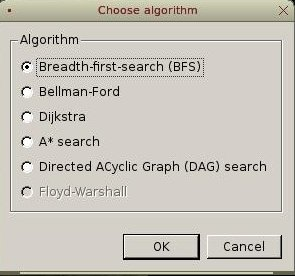
\includegraphics[scale=0.7]{gd1}
    \rule{35em}{0.5pt}
    \caption{Hộp thoại chọn thuật toán}
    \label{fig:AlgorithmChooser}
\end{figure}


    Khi mở chương trình, sẽ có hộp thoại chọn thuật toán
    (\ref{fig:AlgorithmChooser}).\\
\begin{figure}
    \centering
    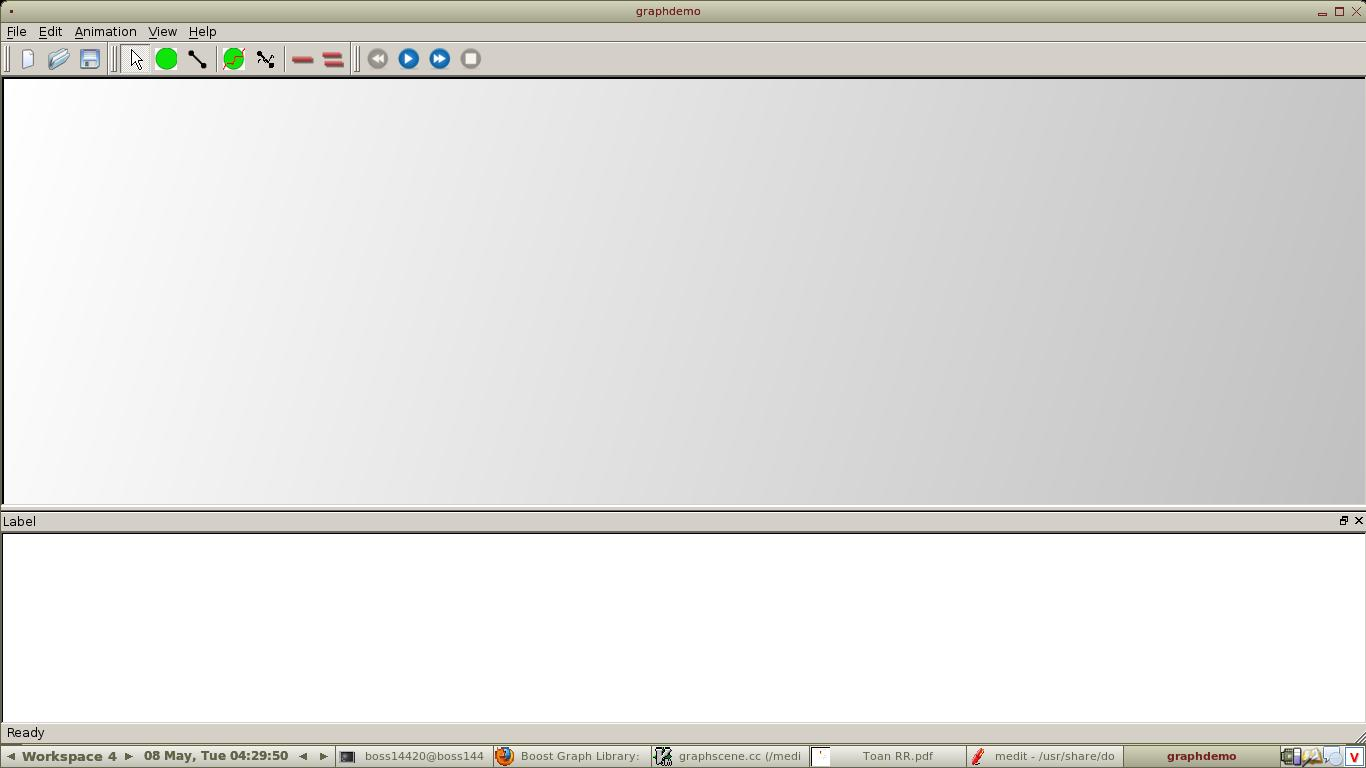
\includegraphics[scale=0.3]{gd2}
    \rule{35em}{0.5pt}
    \caption{Giao diện chính}
    \label{fig:MainWindow}
\end{figure}

\begin{figure}
    \centering
    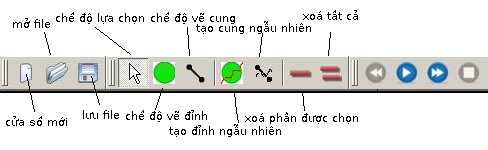
\includegraphics[scale=0.7]{gd3}
    \rule{35em}{0.5pt}
    \caption{Thanh công cụ}
    \label{fig:ToolBars}
\end{figure}

    Sau khi chọn thuật toán, giao diện chính của chương trình hiện ra
    (\ref{fig:MainWindow}).\\
    Để sửa đồ thị, sử dụng thanh công cụ (\ref{fig:ToolBars}) hoặc vào menu.
    Muốn sửa trọng số thì nháy đúp vào trọng số đó.
    Muốn chọn một đỉnh nào đó làm đỉnh nguồn/đích thì click chuột
    phải vào định đó và chọn \textit{Set as source/target}.

    Để bắt đầu chế độ mô phỏng, nhấn nút \textit{Play} hoặc \textit{Next} trên
    thanh công cụ. Ở chế độ này không thể sửa được đồ thị.\\
    Dùng các nút \textit{Next} hoặc \textit{Prev} để tiến/lùi từng bước mô
    phỏng.

\begin{figure}
    \centering
    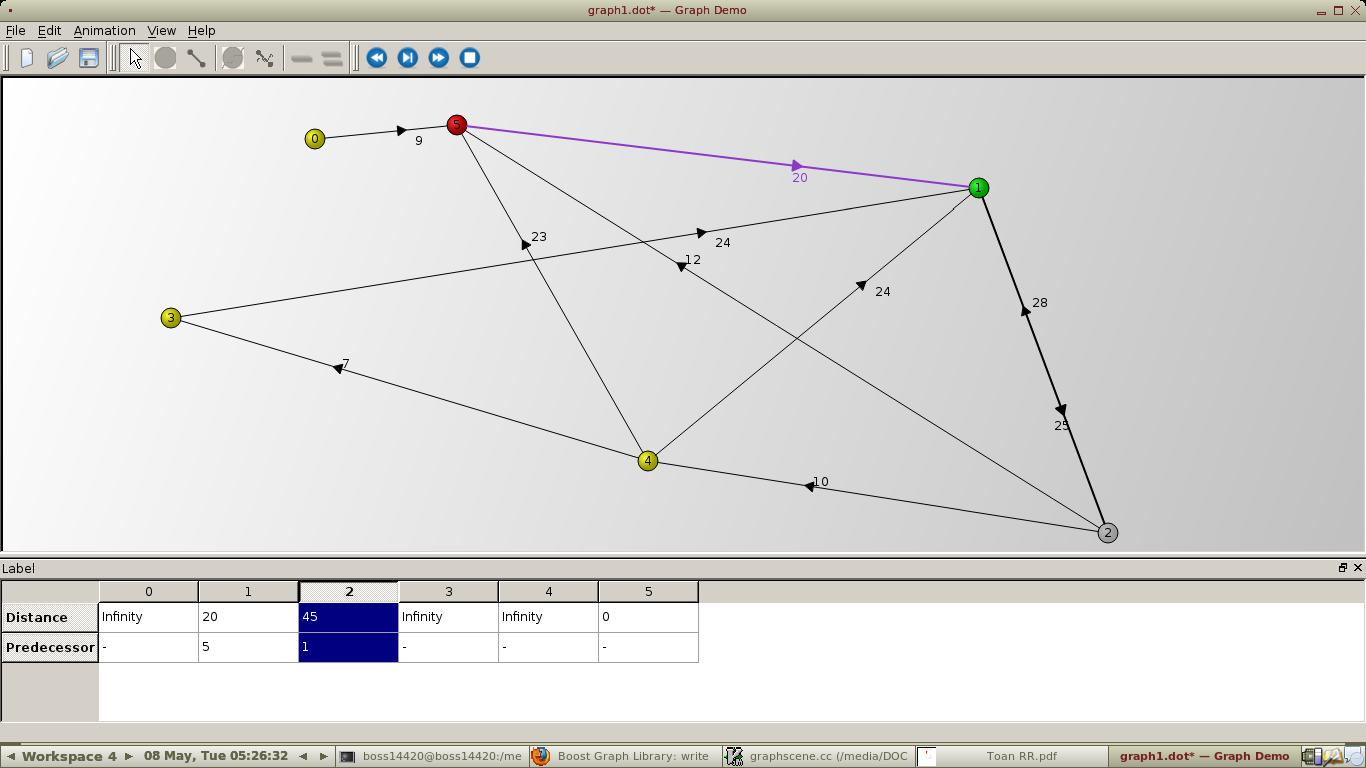
\includegraphics[scale=0.3]{gd4}
    \rule{35em}{0.5pt}
    \caption{Mô phỏng thuật toán Dijkstra}
    \label{fig:Dijkstra1}
\end{figure}
    
    Hình \ref{fig:Dijkstra1}: một bước trung gian trong quá trình tìm kiếm
    bằng thuật toán Dijkstra, trong đó:
    \begin{itemize}
        \item đỉnh màu đỏ là đỉnh nguồn,
        \item đỉnh màu xanh là đỉnh đã được gán nhãn cố định, tức là đã tìm
            được đường đi ngắn nhất từ nguồn đến nó. Ở đây, đỉnh $1$ đã được
            gán nhãn cố định, khoảng cách từ nguồn đến $1$ là $20$.
        \item đỉnh có màu xám là đỉnh đã được \textit{phát hiện (discovered)}
            (có cung nối từ đỉnh màu xanh đến nó) nhưng chưa được gán nhãn cố
            định.
        \item đỉnh màu vàng là đỉnh chưa được xét.
    \end

\begin{figure}
    \centering
    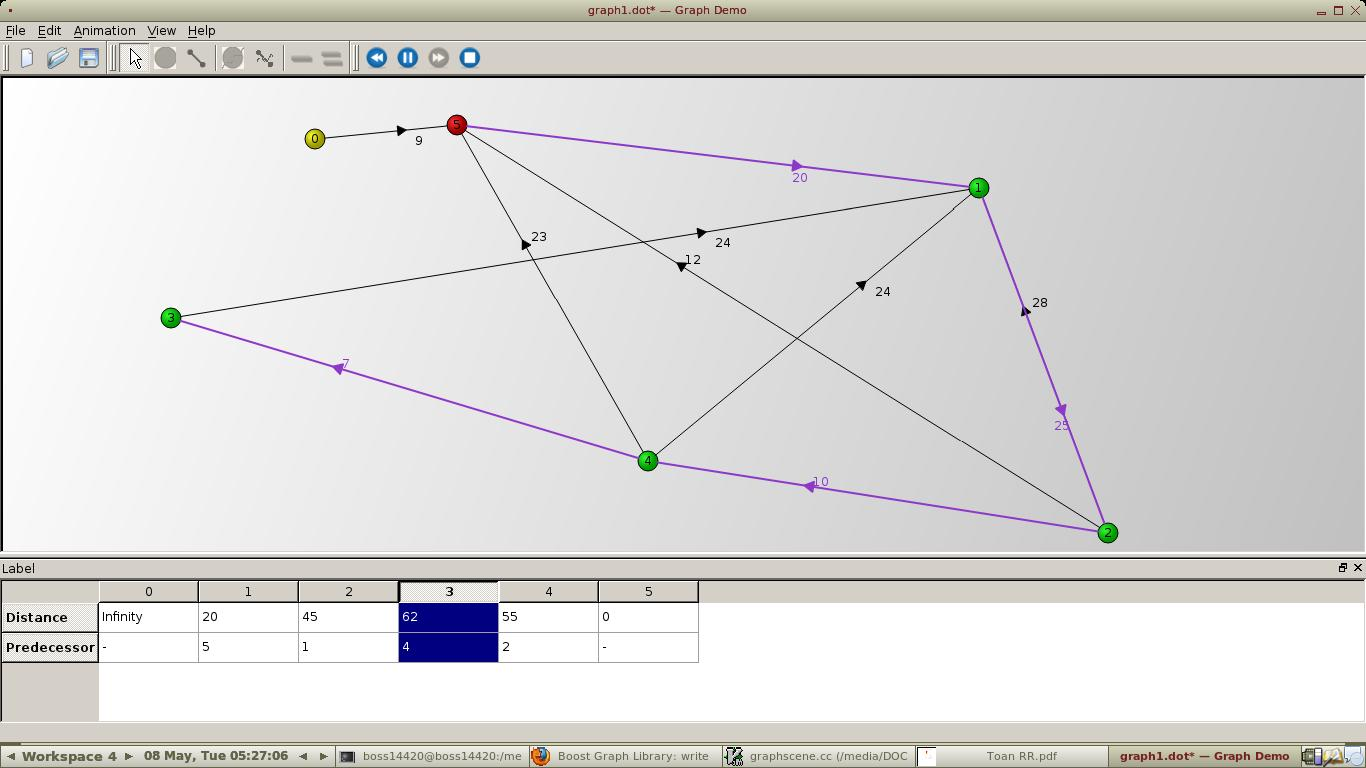
\includegraphics[scale=0.3]{gd5}
    \rule{35em}{0.5pt}
    \caption{Mô phỏng thuật toán Dijkstra}
    \label{fig:Dijkstra2}
\end{figure}
    
    Hình \ref{fig:Dijkstra2}: Kết thúc thuật toán, tất cả các định có thể tới
    từ nguồn có màu xanh (đã tìm được đường đi ngắn nhất), những đỉnh không tìm
    được đường đi ngắn nhất có màu vàng. Những cung màu tím là cung thành phần
    của các đường đi ngắn nhất đã tìm được.\\
    Kết thúc chế độ mô phỏng, nhấn nút \textit{Stop}. Bây giờ có thể tiếp tục
    chỉnh sửa đồ thị.

%========================Phan III================================

%\chapter{Kết luận}

%==================================finish=========================
				
\end{document}
